\documentclass[preview]{standalone}

\usepackage{amsmath}
\usepackage{amssymb}
\usepackage{stellar}
\usepackage{definitions}
\usepackage{graphicx}
\usepackage{tikz}
\usepackage{pgfplots}

\usetikzlibrary{3d, decorations.markings, calc, perspective, shadings, calc, arrows.meta}
\pgfplotsset{compat=1.18}

\tikzset{
    labelstyle/.style={align=center, font=\Large, gray!80!black},
    mathstyle/.style={font=\sffamily\Large\bfseries},
    arrowstyle/.style={->, -Latex, thick, gray!60, shorten >= 3pt, shorten <= 3pt},
    boundarythick/.style={line width=1.5pt}
}

% Identification arrow for the squares to be glued
\tikzset{
    identification arrow/.style={
        postaction={
            decorate,
            decoration={
                markings,
                mark=at position 0.525 with {\arrow[black, scale=1.2, -{Triangle}]{>}}
            }
        }
    }
}

\begin{document}

\genpage{false}

\begin{snippet}{sphere-disk-illustration}
    \begin{center}
        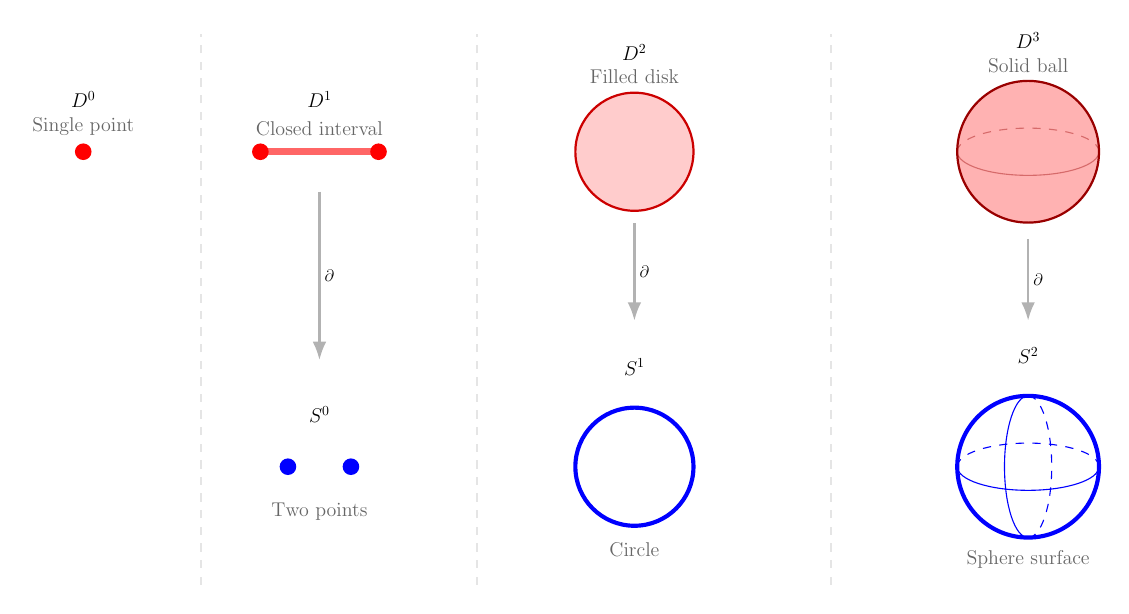
\begin{tikzpicture}[scale=0.5, transform shape, >=Latex]

        \def\toprowy{8cm} 
        \def\bottomrowy{0cm}

        % ================= COLUMN 0: D^0 =================
        \begin{scope}[xshift=0cm]
            % D^0
            \begin{scope}[yshift=\toprowy]
                \fill[red] (0,0) circle (6pt);
                \node[mathstyle, above=1cm] at (0,0) {$D^0$};
                \node[labelstyle, above=0.3cm] at (0,0) {Single point};
            \end{scope}
        \end{scope}

        % ================= COLUMN 1: D^1 and S^0 =================
        \begin{scope}[xshift=6cm]
            % D^1
            \begin{scope}[yshift=\toprowy]
                \draw[line width=2.5pt, red!60] (-1.5,0) -- (1.5,0);
                \fill[red] (-1.5,0) circle (6pt);
                \fill[red] (1.5,0) circle (6pt);
                
                \node[mathstyle, above=1cm] at (0,0) {$D^1$};
                \node[labelstyle, above=0.3cm] at (0,0) {Closed interval};
                
                % Boundary Arrow
                \draw[arrowstyle] (0,-0.8) -- (0,-5.5) node[midway, right, font=\large, black] {$\partial$};
            \end{scope}
            
            % S^0
            \begin{scope}[yshift=\bottomrowy]
                \fill[blue] (-0.8,0) circle (6pt);
                \fill[blue] (0.8,0) circle (6pt);
                \node[mathstyle, above=1cm] at (0,0) {$S^0$};
                \node[labelstyle, below=0.8cm] at (0,0) {Two points};
            \end{scope}
        \end{scope}

        % ================= COLUMN 2: D^2 and S^1 =================
        \begin{scope}[xshift=14cm]
            % D^2
            \begin{scope}[yshift=\toprowy]
                \filldraw[fill=red!20, draw=red!80!black, thick] (0,0) circle (1.5cm);
                
                \node[mathstyle, above=2.2cm] at (0,0) {$D^2$};
                \node[labelstyle, above=1.6cm] at (0,0) {Filled disk};
                
                % Boundary Arrow
                \draw[arrowstyle] (0,-1.6) -- (0,-4.5) node[midway, right, font=\large, black] {$\partial$};
            \end{scope}

            % S^1
            \begin{scope}[yshift=\bottomrowy]
                \draw[boundarythick, blue] (0,0) circle (1.5cm);
                \node[mathstyle, above=2.2cm] at (0,0) {$S^1$};
                \node[labelstyle, below=1.8cm] at (0,0) {Circle};
            \end{scope}
        \end{scope}

        % ================= COLUMN 3: D^3 and S^2 =================
        \begin{scope}[xshift=24cm]
            % D^3
            \begin{scope}[yshift=\toprowy]
                \fill[red!30] (0,0) circle (1.8cm);
                \draw[red!60!black, thick] (0,0) circle (1.8cm);
                
                % 3D Lines
                \draw[red!60!black, thin, opacity=0.4] (-1.8,0) arc (180:360:1.8cm and 0.6cm);
                \draw[red!60!black, thin, dashed, opacity=0.4] (1.8,0) arc (0:180:1.8cm and 0.6cm);
                
                \node[mathstyle, above=2.5cm] at (0,0) {$D^3$};
                \node[labelstyle, above=1.9cm] at (0,0) {Solid ball};
                
                % Boundary Arrow
                \draw[arrowstyle] (0,-2.0) -- (0,-4.5) node[midway, right, font=\large, black] {$\partial$};
            \end{scope}

            % S^2
            \begin{scope}[yshift=\bottomrowy]
                \draw[boundarythick, blue] (0,0) circle (1.8cm);
                \draw[blue, thin] (-1.8,0) arc (180:360:1.8cm and 0.6cm);
                \draw[blue, thin, dashed] (1.8,0) arc (0:180:1.8cm and 0.6cm);
                \draw[blue, thin] (0,1.8) arc (90:270:0.6cm and 1.8cm);
                \draw[blue, thin, dashed] (0,-1.8) arc (-90:90:0.6cm and 1.8cm);
                
                \node[mathstyle, above=2.5cm] at (0,0) {$S^2$};
                \node[labelstyle, below=2.0cm] at (0,0) {Sphere surface};
            \end{scope}
        \end{scope}

        % --- Separators ---
        \draw[gray!20, dashed, thick] (3, -3) -- (3, 11);
        \draw[gray!20, dashed, thick] (10, -3) -- (10, 11);
        \draw[gray!20, dashed, thick] (19, -3) -- (19, 11);

        \end{tikzpicture}
    \end{center}
\end{snippet}

\begin{snippet}{cylinder-illustration-gluing}
    \begin{center}
        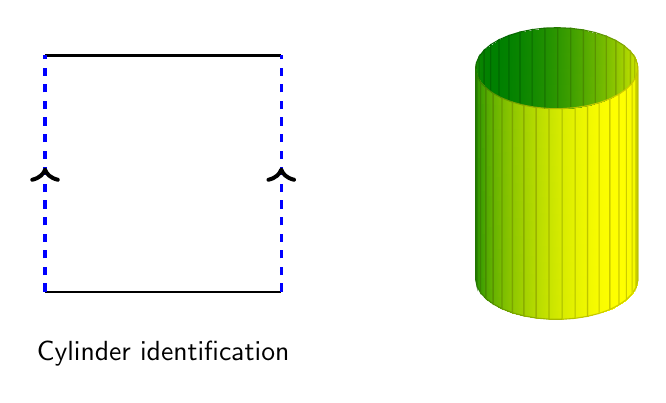
\begin{tikzpicture}
            % --- LEFT SIDE: Identification Square ---
            \begin{scope}[xshift=-6.5cm, yshift=1cm]
                % Coordinates
                \coordinate (BL) at (0,0);
                \coordinate (BR) at (3,0);
                \coordinate (TR) at (3,3);
                \coordinate (TL) at (0,3);

                % 1. Horizontal lines (Boundaries) - Solid
                \draw[thick] (BL) -- (BR);
                \draw[thick] (TL) -- (TR);

                % 2. Vertical lines (Glued edges) - Dashed Blue
                % Left edge: Arrow pointing UP
                \draw[very thick, dashed, blue, identification arrow] (BL) -- (TL);

                % Right edge: Arrow pointing UP
                % NOTE: For a cylinder, the arrows must point in the SAME direction.
                % We draw from Bottom-Right (BR) to Top-Right (TR) to make the arrow point up.
                \draw[very thick, dashed, blue, identification arrow] (BR) -- (TR);

                % Label
                \node[below=0.5cm, font=\sffamily] at (1.5,0) {Cylinder identification};
            \end{scope}

            % --- RIGHT SIDE: PGFPlots Cylinder ---
            \begin{axis}[
                yshift=2.5cm,
                anchor=center,
                hide axis,
                view={40}{30}, % Slightly lower angle to see the tube shape better
                width=8cm, height=8cm,
                axis equal,
                /tikz/background rectangle/.style={fill=none}
            ]
                % The Cylinder Surface
                \addplot3 [
                    surf,
                    shader=faceted interp,
                    point meta=x,
                    colormap/greenyellow,
                    samples=40,     % Resolution around the circle
                    samples y=2,    % Resolution along the height (cylinder is straight, so 2 is enough)
                    z buffer=sort,
                    domain=0:360,   % Angle (theta)
                    y domain=-1.5:1.5, % Height (z) - Taller than the strip to look like a tube
                    thin
                ] (
                    {cos(x)}, % x = r*cos(theta)
                    {sin(x)}, % y = r*sin(theta)
                    {y}       % z = height
                );
            \end{axis}
        \end{tikzpicture}
    \end{center}
\end{snippet}

\begin{snippet}{torus-surface-illustration-gluing}
    \begin{center}
        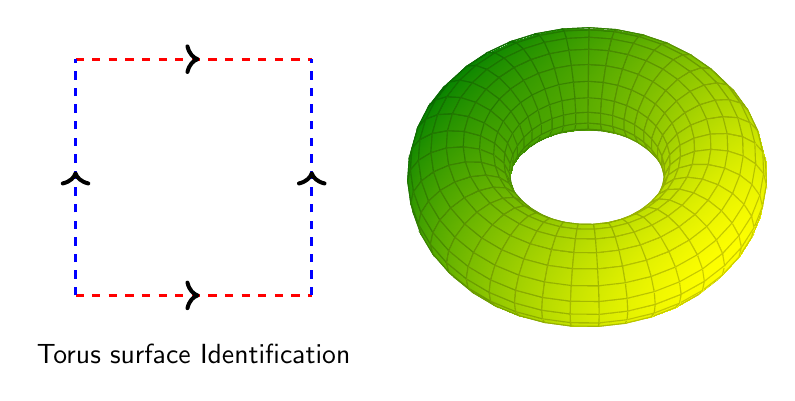
\begin{tikzpicture}
            \begin{scope}[xshift=-6.5cm, yshift=1cm]
                % Coordinates
                \coordinate (BL) at (0,0);
                \coordinate (BR) at (3,0);
                \coordinate (TR) at (3,3);
                \coordinate (TL) at (0,3);

                \draw[very thick, dashed, red, identification arrow] (BL) -- (BR);
                \draw[very thick, dashed, red, identification arrow] (TL) -- (TR);

                \draw[very thick, dashed, blue, identification arrow] (BL) -- (TL);
                \draw[very thick, dashed, blue, identification arrow] (BR) -- (TR);

                \node[below=0.5cm, font=\sffamily] at (1.5,0) {Torus surface Identification};
            \end{scope}

            \begin{axis}[
                yshift=2.5cm,
                anchor=center,
                hide axis,
                view={40}{50}, % Higher angle to see the hole clearly
                width=8cm, height=8cm,
                axis equal,
                /tikz/background rectangle/.style={fill=none}
            ]
                % The Torus Surface
                \addplot3 [
                    surf,
                    shader=faceted interp,
                    point meta=x,
                    colormap/greenyellow,
                    samples=40,    % Resolution around the ring (u)
                    samples y=20,  % Resolution of the tube cross-section (v)
                    z buffer=sort,
                    domain=0:360,  % u
                    y domain=0:360,% v
                    thin
                ] (
                    {(1 + 0.4*cos(y))*cos(x)}, % x
                    {(1 + 0.4*cos(y))*sin(x)}, % y
                    {0.4*sin(y)}               % z
                );
            \end{axis}
        \end{tikzpicture}
    \end{center}
\end{snippet}

\begin{snippet}{mobius-strip-illustration-gluing}
    \begin{center}
        % https://tex.stackexchange.com/questions/118563/moebius-strip-using-tikz
        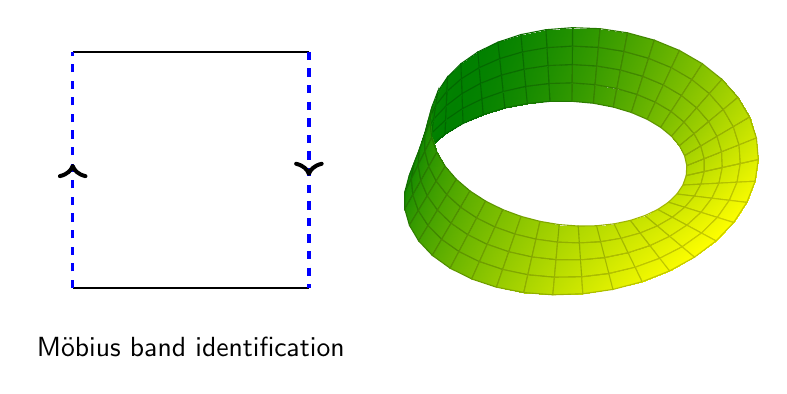
\begin{tikzpicture}
            \begin{scope}[xshift=-6.5cm, yshift=1cm]
                \coordinate (BL) at (0,0);
                \coordinate (BR) at (3,0);
                \coordinate (TR) at (3,3);
                \coordinate (TL) at (0,3);
                \draw[thick] (BL) -- (BR);
                \draw[thick] (TL) -- (TR);
                \draw[very thick, dashed, blue, identification arrow] (BL) -- (TL);
                \draw[very thick, dashed, blue, identification arrow] (TR) -- (BR);
                \node[below=0.5cm, font=\sffamily] at (1.5,0) {Möbius band identification};
            \end{scope}

            \begin{axis}[
                yshift=2.5cm,
                anchor=center, % Anchor at the center of the plot
                hide axis,
                view={40}{40},
                width=8cm, height=8cm,
                axis equal,
                /tikz/background rectangle/.style={fill=none}
            ]
                % The Surface
                \addplot3 [
                    surf,
                    shader=faceted interp,
                    point meta=x,
                    colormap/greenyellow,
                    samples=40,
                    samples y=5,
                    z buffer=sort,
                    domain=0:360,
                    y domain=-0.5:0.5,
                    thin
                ] (
                    {(1+0.5*y*cos(x/2))*cos(x)},
                    {(1+0.5*y*cos(x/2))*sin(x)},
                    {0.5*y*sin(x/2)}
                );
            \end{axis}
        \end{tikzpicture}
    \end{center}
\end{snippet}

\begin{snippet}{klein-bottle-illustration-gluing}
    \begin{center}
        \begin{tikzpicture}
            \begin{scope}[xshift=0cm, yshift=0cm]
                \coordinate (BL) at (0,0); % Bottom Left
                \coordinate (BR) at (3,0); % Bottom Right
                \coordinate (TR) at (3,3); % Top Right
                \coordinate (TL) at (0,3); % Top Left

                \draw[very thick, dashed, red, identification arrow] (BL) -- (BR);
                \draw[very thick, dashed, red, identification arrow] (TR) -- (TL);

                \draw[very thick, dashed, blue, identification arrow] (BL) -- (TL);
                \draw[very thick, dashed, blue, identification arrow] (BR) -- (TR);

                \node[below=0.5cm, font=\sffamily] at (1.5,0) {Klein's bottle identification};
            \end{scope}
            \node[anchor=west] at (4.5, 1.5) {
                \includegraphics[width=4cm]{resources/klein.png}
            };
        \end{tikzpicture}
    \end{center}
\end{snippet}

\begin{snippet}{genus-two-torus-illustration}
    \begin{center}
        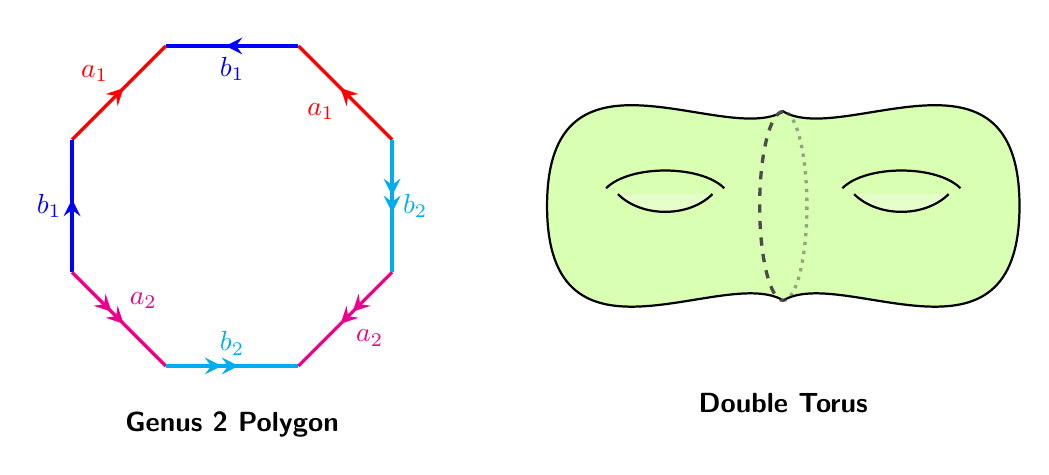
\begin{tikzpicture}
            \tikzset{
                mid arrow/.style={
                    postaction={
                        decorate,
                        decoration={
                            markings,
                            mark=at position 0.55 with {\arrow[scale=1.2, >=stealth]{>}}
                        }
                    }
                },
                mid double arrow/.style={
                    postaction={
                        decorate,
                        decoration={
                            markings,
                            mark=at position 0.55 with {\arrow[scale=1.2, >=stealth]{>>}}
                        }
                    }
                }
            }

            % --- LEFT SIDE: Identification Octagon ---
            \begin{scope}[xshift=-7cm, yshift=2.5cm]
                % Define the radius of the octagon
                \def\R{2.2}
                
                % Calculate vertices of a regular octagon
                % We rotate by 22.5 degrees so it has flat vertical/horizontal sides (Stop sign shape)
                \foreach \i in {1,...,8} {
                    \coordinate (P\i) at ({22.5 + (\i-1)*45}:\R);
                }

                % --- DRAWING THE EDGES ---
                % The sequence for a genus 2 surface is usually: a1 b1 a1^-1 b1^-1 a2 b2 a2^-1 b2^-1
                
                % HANDLE 1 (Red & Blue, Single Arrows)
                % a1
                \draw[very thick, red, mid arrow] (P1) -- (P2) node[midway, auto] {$a_1$};
                % b1
                \draw[very thick, blue, mid arrow] (P2) -- (P3) node[midway, auto] {$b_1$};
                % a1 inverse (Arrow points backwards relative to the walk)
                \draw[very thick, red, mid arrow] (P4) -- (P3) node[midway, auto] {$a_1$};
                % b1 inverse
                \draw[very thick, blue, mid arrow] (P5) -- (P4) node[midway, auto] {$b_1$};

                % HANDLE 2 (Magenta & Cyan, Double Arrows to distinguish)
                % a2
                \draw[very thick, magenta, mid double arrow] (P5) -- (P6) node[midway, auto] {$a_2$};
                % b2
                \draw[very thick, cyan, mid double arrow] (P6) -- (P7) node[midway, auto] {$b_2$};
                % a2 inverse
                \draw[very thick, magenta, mid double arrow] (P8) -- (P7) node[midway, auto] {$a_2$};
                % b2 inverse
                \draw[very thick, cyan, mid double arrow] (P1) -- (P8) node[midway, auto] {$b_2$};

                % Label
                \node[below=2.5cm, font=\sffamily\bfseries] at (0,0) {Genus 2 Polygon};
            \end{scope}

            % --- RIGHT SIDE: The Double Torus (Constructed via Bezier curves) ---
            % Parametric plotting of a genus 2 surface is unstable in pure LaTeX.
            % We draw it constructively to ensure it looks perfect.
            \begin{scope}[xshift=0cm, yshift=2.5cm, scale=1.5]
                
                % Colors mimicking the surface plots
                \colorlet{surfColor}{green!50!yellow!30}
                \colorlet{shadeColor}{green!30!yellow!60!black}

                % 1. The Main Outline (The Peanut)
                \draw[fill=surfColor, thick] 
                    (-2,0) .. controls (-2,1.5) and (-0.5, 0.5) .. (0, 0.8) % Top Left Hump
                        .. controls (0.5, 0.5) and (2,1.5) .. (2,0)      % Top Right Hump
                        .. controls (2,-1.5) and (0.5, -0.5) .. (0, -0.8)% Bottom Right Hump
                        .. controls (-0.5, -0.5) and (-2,-1.5) .. (-2,0);% Bottom Left Hump

                % 2. The "Holes" (Visualized as curves)
                % Left Hole
                \draw[thick, fill=white, fill opacity=0.3] 
                    (-1.4, 0.1) .. controls (-1.2, -0.1) and (-0.8, -0.1) .. (-0.6, 0.1); % Smile
                \draw[thick] 
                    (-1.5, 0.15) .. controls (-1.3, 0.35) and (-0.7, 0.35) .. (-0.5, 0.15); % Frown

                % Right Hole
                \draw[thick, fill=white, fill opacity=0.3] 
                    (0.6, 0.1) .. controls (0.8, -0.1) and (1.2, -0.1) .. (1.4, 0.1); % Smile
                \draw[thick] 
                    (0.5, 0.15) .. controls (0.7, 0.35) and (1.3, 0.35) .. (1.5, 0.15); % Frown

                % 3. The "Cut" in the middle
                % This is the connected sum boundary.
                % Drawn as a dashed ellipse wrapping around the "waist"
                \draw[very thick, dashed, black!70] (0, 0.8) arc (90:270:0.2 and 0.8);
                \draw[very thick, dotted, black!70, opacity=0.5] (0, -0.8) arc (-90:90:0.2 and 0.8);

                % Label
                \node[below=1.5cm, font=\sffamily\bfseries] at (0,-0.5) {Double Torus};
            \end{scope}
        \end{tikzpicture}
    \end{center}
\end{snippet}

\end{document}